\section{Preliminaries}
\label{Appendix: DER}
% \begin{wrapfigure}{R}{0.45\textwidth} 
%     \vspace*{-1.0cm}
%     \centering
%      \includegraphics[width=0.42\textwidth]{figures/DlO.PNG}
%      \caption{A Deformable Linear Object (DLO) model that describes the notation used throughout the paper.}
%     \label{fig:DLO}
%     \vspace*{-1.1cm}
% \end{wrapfigure}
This section introduces the key components of DER models while describing their limitations.
Note that more details about DER can be found at \cite{originalDER}. \Revise{We also introduce existing state estimation algorithms of DLOs and discuss potential improvements.}{}% Throughout the rest of the document, let  $|\cdot|$ represents $||\cdot||_2$ and $\times$ denote the cross product between two vectors in $\R^3$.
 \subsection{Deformable Linear Object (DLO) Model}
To model a DLO, we separate the DLO into an indexed set of $n$ vertices at each time instance. 
The ground truth locations of vertex $i$ at time $t$ is denoted by $\timevertind{x}{i}{t} \in \R^3$ and the set of all $n$ vertices is denoted by $\timeind{X}{t}$ as illustrated in Figure \ref{fig:DLO}. 
Let $\textit{\textbf{M}}^\text{i}\in \mathbb{R}^{3\times3}$ denote the mass matrix of vertex $i$.
A segment, or edge, in the DLO is the line between successive vertices, $\timevertind{e}{i}{t} = \timevertind{x}{i+1}{t} - \timevertind{x}{i}{t}$.
Let $\timeind{E}{t}$ correspond to the set of all edges at time $t$.
Our objective is to model the dynamic behavior of a DLO that is being controlled by a robot and as a result we make the following assumption:
\begin{assum}
    The first and last edge of the DLO are each held by a distinct end effector of a robot 
    \label{assum:grasp condition}
\end{assum}
Note this assumption is commonly made during DLO manipulation \cite{IRP, diminishingridgidity, directionalrigidity, inlstm, gelsim}. Using this assumption, let the orientation and position of the two end effectors at time $t$ be denoted by $\vertindu_t \in \R^{12}$, which we refer to as the input.
Let $\textbf{U}_{1:\text{T}-1}$ denote the set of inputs applied between times $t=1$ and $t=\text{T}-1$, and let $\textbf{X}_{1:\text{T}} =\{\textbf{X}_1, \textbf{X}_2,\ldots, \textbf{X}_\text{T}\} \in \mathbb{R}^{\text{T} \times \text{n}\times 3}$ denote the associated trajectory of the DLO from times $t=1$ to $t=\text{T}$.

Let $\Delta_t$ denote the difference in time between successive elements of $\textbf{X}_{1:\text{T}}$.
Then, the velocity of the vertices of the DLO can be denoted as $\timeind{V}{t}  = (\timeind{X}{t} - \timeind{X}{t-1})/\Delta \text{t}$.
Finally, note that we distinguish between ground truth elements and predicted elements by using the circumflex symbol (\textit{e.g.}, $\textbf{X}_{t}$ is the ground truth set of vertices at time $t$ and $\pred{X}{t}$ is the predicted set of vertices at time $t$).

\subsection{Modeling DLO with DER for Dual Manipulation}
\label{sec:DER}

DLOs primarily exhibit three distinct modes: bending, twisting, and stretching \cite{originalDER}. 
% \Zac{is modes the word used by the cited paper? I feel like deformation modes makes sense for the first two, but not inextensibility. maybe change inextensibility to stretching.} \Yizhou{I think it might be ok to keep this? otherwise we need to have another sentence to connect stretching and inextensibility?}
In this paper, we focus on DLOs that are inextensible, and therefore do not experience stretching.
Accurately modeling the bending and twisting modes of a DLO is challenging without introducing a large number of parameters.
Unfortunately, the behavior of a model with large numbers of parameters is challenging to simulate in real-time \cite{twistbendchallenge, twistbendchallenge2}.
To enforce inextensibility, it is typical to apply a large stretch stiffness, but this can introduce instabilities during simulation, making these models difficult to use for prediction.
To address these challenges, (1) DER introduces a single scalar $\theta^\text{i}_{t} \in \R$ that accurately represents bending and twisting in $\R^3$ and (2) DER enforces inextensibility using a fast, stable projection method \cite[Section 4]{fast_proj}. 

\subsection{Potential Energy to Equations of Motion} 

A DLO can be modeled using DER by first introducing a family of frames that are collocated with each of the vertices. 
In particular, each frame's relationship with the prior frame is parameterized by $\theta^\text{i}_t \in \R$.
An explanation for why a single scalar is sufficient to describe this rotation can be found in \cite[Section 4.2]{originalDER}.
If one is given $\textbf{X}_t$, then one can compute $\theta^\text{i}_t$.
As a result, we write $\bm{\theta}_t(\textbf{X}_t)$ to denote the vector of all $\theta^\text{i}_t$ at a time $t$.
Note, we explain how to compute $\bm{\theta}_t(\textbf{X}_t)$ before the end of this section.

Using this representation, DER is able to accurately approximate the potential energy of the DLO that arises due to bending or twisting. 
This potential energy is a function of the material properties of each vertex of the DLO (i.e., their mass, bending modulus, and twisting modulus) and the configuration of the DLO.
If we let $\bm{\alpha}$ denote the vector of the material properties of each vertex of the DLO, then one can write down the potential energy of a particular configuration of the DLO as $P(\textbf{X}_t, \bm{\theta}_t(\textbf{X}_t),\bm{\alpha})$ \cite[Section 4.2]{originalDER}.

Once the potential energy expression is derived, then the restorative force experienced during deformation is equal to the negative of the gradient of the potential energy expression with respect to the vertices. Therefore, the equation of motion of the DLO is:
\begin{equation}
       \textit{\textbf{M}}\ddot{\textbf{X}}_{t} = -\frac{\partial P(\textbf{X}_t, \bm{\theta}_t(\textbf{X}_t),\bm{\alpha})}{\partial  \textbf{X}_{t}}
       \label{eq:Integration}
\end{equation}
One can numerically integrate this formula to predict the velocity and position by applying the Semi-Implicit Euler method:
\begin{align}
        \hat{\textbf{V}}_{t+1} &= \hat{\textbf{V}}_\text{t}-\Delta_\text{t}M^{-1}\frac{\partial P(\hat{\textbf{X}}_t, \bm{\theta}_t(\hat{\textbf{X}}_t),\bm{\alpha})}{\partial \textbf{X}_{t}}, \label{eq:Semi-Euler1}\\  
        \hat{\textbf{X}}_{\text{t}+1} &= \hat{\textbf{X}}_\text{t} + \Delta_\text{t}\hat{\textbf{V}}_{t+1}.
       \label{eq:Semi-Euler2}
\end{align}

One can use \eqref{eq:Semi-Euler1}-\eqref{eq:Semi-Euler2} with state-of-the-art ODE solvers to simulate the behavior of the DER model of a DLO.
However, computing the gradient of the potential energy requires an expression for $\bm{\theta}_t(\textbf{X}_t)$. 
To construct such an expression, DER assumes that the DLO reaches an equilibrium state between each simulation time step:
\begin{assum}
    Between each step of the simulation, the DLO reaches an equilibrium state. 
    As a result, at each time step $t$, one can compute
    \begin{equation}
        \bm{\theta}^*_t(\textbf{X}_t) = \argmin_{\bm{\theta}_t} P(\textbf{X}_t, \bm{\theta}_t,\bm{\alpha})
        \label{eq:opt_theta}
    \end{equation}
\end{assum}
To summarize, at each integration time step, one must solve \eqref{eq:opt_theta} to evaluate the dynamics. 
There are several factors which make simulating this model  quickly and accurately challenging.
First, it may be difficult to accurately estimate the material properties of an arbitrary DLO before simulating the model. 
In \secref{sec:Differentiable DER}, we illustrate how to make the DER model differentiable so that one can estimate the material properties from real-world data while simulating the model.
Second, there is an undesirable tradeoff between choosing a larger time step to achieve real-time prediction and the accuracy of that prediction.
In \secref{sec:integration_NN}, we apply residual learning to perform predictive compensation during integration which enables rapid simulation of the model without sacrificing accuracy.


\subsubsection{Inextensibility Enforcement}
During simulation, the DLO's length may change due to numerical errors, but this is undesirable when modeling DLOs like cables and ropes, which are inextensible.
To ensure that the length of the DLO does not change during simulation, DER methods project a computed solution onto a constraint set that ensures that the DLO's length does not change.
% \begin{equation}
%     \textbf{e}_\text{i} \cdot \textbf{e}_\text{i} - \overline{\textbf{e}}_\text{i}\cdot\overline{\textbf{e}}_\text{i} = 0
% \label{eq:inextensibility}
% \end{equation}
% where $\overline{\textbf{e}}_\text{i}$ denotes the undeformed edge. 
However, this projection operation can introduce instabilities during simulation because it does not ensure that momentum is conserved during motion.
This papers adopts a constraint solver based on a PBD model \cite{PBD}, which is described in Section \ref{sec:inextensiblity methodology}, to enforce inextensiblity while conserving momentum.
This improves the accuracy of prediction when compared to classical methods. 

% \begin{wrapfigure}{R}{0.6\textwidth}
%       \vspace*{-0.65cm}
%     \begin{minipage}{0.6\textwidth}
%       \begin{algorithm}[H]
% \caption{One Step Prediction} 
% \label{alg:long time horizon}
% \textbf{Inputs}: $\pred{X}{t}, \pred{V}{t}, \textbf{u}_t$
% \begin{algorithmic}[1]
% % \State Align end edges with $\textbf{u}_t$ \Comment{assumption.\ref{assum:grasp condition}}
% \State $\bm{\theta}^*_t(\textbf{X}_t) = \argmin_{\bm{\theta}_t} P(\textbf{X}_t, \bm{\theta}_t,\bm{\alpha})$ \Comment{\secref{sec:Differentiable DER}}
% % \State  $\textit{\textbf{M}}\ddot{\textbf{X}}_{t} = -\frac{\partial P(\textbf{X}_t, \bm{\theta}_t(\textbf{X}_t),\bm{\alpha}}{\partial  \textbf{X}_{t}}$
% % \Comment{\eqref{eq:Integration}} 
% \State $\hat{\textbf{V}}_{t+1} = \hat{\textbf{V}}_t-\Delta_tM^{-1}\frac{\partial P(\textbf{X}_t, \bm{\theta}^*_t(\textbf{X}_t),\bm{\alpha})}{\partial \textbf{X}_{t}}$ \Comment{\eqref{eq:Semi-Euler2}}   
% \State $\hat{\textbf{X}}_{t+1} = \hat{\textbf{X}}_t + \Delta_t\hat{\textbf{V}}_{t+1} + \text{DNN}$ \Comment{\secref{sec:integration_NN}}
% \State Inextensibility Enforcement on $\hat{\textbf{X}}_{t+1}$ 
% \Comment{\secref{sec:inextensiblity methodology}}
% \State $\hat{\textbf{V}}_{t+1} = (\hat{\textbf{X}}_{t+1} - \hat{\textbf{X}}_t)\Delta_t$ \Comment{Velocity Update}
% \end{algorithmic}
% \Return $\pred{X}{t+1}, \pred{V}{t+1}$
% \end{algorithm}
%     \end{minipage}
%   \end{wrapfigure}

% \begin{wrapfigure}{R}{0.44\textwidth}
% \vspace*{-0.65cm}
%     \begin{minipage}{0.44\textwidth}
% \begin{algorithm}[H]
% \caption{Enforcing Inextensibility with Momentum Preserving PBD} 
% \label{alg:inextensibility of PBD}
% \begin{algorithmic}[1]
% \Require $\pred{X}{t+1}$ and $\epsilon > 0$
% \While {any $\text{C}(\hat{\textbf{x}}^i_{t+1}, \hat{\textbf{x}}^{i+1}_{t+1}) > \epsilon$ }
%     \For{$i = 2$ \textbf{to} $n - 1$}
%         \State $\hat{\textbf{x}}_{t+1}^i = \hat{\textbf{x}}_{t+1}^i + \beta^{i}\Delta \hat{\textbf{x}}_{t+1}^i$ \Comment{\eqref{eq:inext1}}
%         % \State $\hat{\textbf{x}}_{t+1}^\text{i+1} = \hat{\textbf{x}}_{t+1}^\text{i+1} + \beta^{i+1}\Delta \hat{\textbf{x}}_{t+1}^\text{i+1}$ \Comment{\eqref{eq:inext1}}   
%     \EndFor
% \EndWhile
% % \Until{\textbf{all} $||\hat{\textbf{x}}_{t+1}^i - \hat{\textbf{x}}_{t+1}^\text{i+1}|| - ||\overline{\textbf{e}}_i||_2 < threshold$}
% \State \Return: $\hat{\textbf{X}}_{t+1}$ \Comment{Updated Vertices}
% \end{algorithmic}
% \end{algorithm}
% \end{minipage}
%   \end{wrapfigure}

% \begin{table}[t]
% \centering
% \caption{A summary of the material properties of each of the wires that were observed/manipulated during the real-world experiment.}
% \label{mat_prop}
% \begin{tabular}{|c||c|c|c|c|}
% \hline
% Name & Length [m] & Weight [g] & Stiffness & \makecell{ \# Mocap \\ Markers}\\ \hline \hline
% DLO 1 & 1.152 & 34.5 & 3 & 13\\ \hline 
% DLO 2 & 0.996 & 65.2 & 4 & 12\\ \hline 
% DLO 3 & 0.998 & 96.8  & 5 & 12 \\ \hline
% DLO 4& 0.973 & 22.0 & 1 & 12\\ \hline 
% DLO 5 & 0.988 & 19.2 & 2 & 12 \\ \hline 
% \end{tabular}
% \end{table}
% \subsection{\Review{}{Motion Planning and Control for DLO Manipulation}{}}



% However, based on experiment and natural deficiency from large-time step discretization, we find that this method cannot capture high dynamic performance. 
% We enhance the integration approach by incorporating predictive compensation. 
% This enhancement is rooted in the concept of residual learning and is achieved through the adaptation of a graph neural network. 
% Further details will be discussed in \secref{sec:integration_NN}.
% ; however, note that our goal is to eventually perform differentiable simulation to allow for auto-tuning certain model parameters which is described in more detail in \secref{sec:Differentiable DER}.

% \subsection{Long Time Horizon Prediction for DLO}

% Following assumptions are made to setup a prediction framework.
% \begin{assum}
%     first two states $\timeind{X}{1}, \timeind{X}{2}$ are fully observable. 
% \end{assum}
% Satisfying this assumption is essential for the initialization of iterative prediction. However, when perception is heavily occluded at the initial state, meeting above assumption can be challenging. Details will be discussed in \secref{section: Estimation}
% \begin{assum}
% End edges of DLO are coupled with grippers such that $\textbf{u}_\text{t}=\{\timevertind{x}{1}{t+1}, \timevertind{x}{2}{t+1}, \timevertind{x}{n-1}{t+1}, \timevertind{x}{n}{t+1}\}$. $\textbf{u}_\text{t}$ can be approximated through inverse kinematics or other perception system.
% \end{assum}
% Above assumption commonly made and well-studied in DLO manipulation among literature\cite{IRP, diminishingridgidity, directionalrigidity, inlstm, gelsim}. It provides accessibility and controllability to DLO edges.

%  \Ram{use an assumption environment like in the file I shared with you....} 
% \Ram{what does this mean?}. With above assumptions, denote $F$ as a general modeling function, long-time horizon inference is propagated through iterative prediction as shown in the \textbf{Algorithm} \ref{alg:long time horizon}. Note ground truth is not accessible during the iteration, and all predicted intermediate and final states of the DLO will be used for evaluation. 
% \begin{algorithm}[t]
% \caption{Long Time Horizon Prediction } 
% \label{alg:long time horizon}
% \textbf{Require:} $\textbf{X}_{1:\text{T}}, \textbf{U}_{2:\text{T-1}}$ \Comment{True States and Inputs}\\
% \textbf{Initialization} at t = 2: 
% \begin{algorithmic}[1]
% \State $\textbf{V}_2 = (\textbf{X}_2 - \textbf{X}_1)/\Delta \text{t}$ \Comment{Initial Velocity Estimation } 
% \State $\pred{X}{3} = F(\textbf{u}_2, \textbf{X}_2, \textbf{V}_2)$   \Comment{First Update}
% \State $\pred{V}{3} = (\pred{X}{3} - \textbf{X}_2)/\Delta \text{t}$ \Comment{Velocity Update}
% \State {Iterative Update: $\text{T} \gg \Delta \text{t}$ \Ram{not sure why you need this condition...I think you are just running a for loop? Also isn't this just a single algorithm, why does the line number change halfway thru? Is this supposed to be two algorithms? Then call them two algorithms?}} \Yizhou{I was trying to show it is long time horizon but I can delete this line.}
% \For{$\text{t} \gets 3 \textrm{ to } \text{T}-1$} 
%      \State $\pred{X}{t+1} = F(\textbf{u}_\text{t}, \pred{X}{t}, \pred{V}{t})$
%      \State $\pred{V}{t+1} = (\pred{X}{t+1} - \pred{X}{t})/\Delta t$
% \EndFor
% \State \Return $\pred{X}{3:T}, \, |\pred{X}{3:T} - \timeind{X}{3:T}|$ \Comment{Prediction and Loss}
% \end{algorithmic}
% \end{algorithm}


% \subsection{Integration for DLO Simulation}
% \label{sec:integration}
% Notice that $\theta^*_\text{t}$ is a function of $\timeind{X}{t}$. For conciseness, based on \Eqref{eq:energy}, we note equation of motion as follows: 
% \begin{equation}
%        \textit{\textbf{M}}\ddot{\textbf{X}}_{t} = -\frac{\delta \text{E}(\Gamma^\text{M}(\timeind{X}{t}))}{\delta \textbf{X}_{t}}
%        \label{eq:Integration}
% \end{equation}
% As DER is not an analytical modeling frame. Solving  \Eqref{eq:Integration} requires numerical integration. DER\cite{originalDER} choose the method to be Semi-Euler method\cite{implicit-euler}, which has the same computational cost while having better tracking performance compared to Euler's method, as shown in the following, 
% \begin{equation}
%         \hat{\textbf{V}}_{t+1} = \textbf{V}_\text{t} -\Delta \text{t}m^{-1}\frac{\delta \text{E}(\Gamma^\text{M}(\textbf{X}_{t}))}{\delta \textbf{X}_{t}}, \, \,  \hat{\textbf{X}}_{\text{t}+1} = \textbf{X}_\text{t} + \Delta \text{t} \hat{\textbf{V}}_{t+1}
%        \label{eq:Semi-Euler}
% \end{equation}
% However, based on experiment and natural deficiency from large-time step discretization, we find that this method cannot capture high dynamic performance. We enhance the integration approach by incorporating predictive compensation. This enhancement is rooted in the concept of residual learning and is achieved through the adaptation of a graph neural network. Further details will be discussed in \secref{sec:integration_NN}.

% \subsection{Long Time Horizon Prediction for DLO}
% Following assumptions are made to setup a prediction framework.
% \begin{assum}
%     first two states $\timeind{X}{1}, \timeind{X}{2}$ are fully observable. 
% \end{assum}
% Satisfying this assumption is essential for the initialization of iterative prediction. However, when perception is heavily occluded at the initial state, meeting above assumption can be challenging. Details will be discussed in \secref{section: Estimation}
% \begin{assum}
% End edges of DLO are coupled with grippers such that $\textbf{u}_\text{t}=\{\timevertind{x}{1}{t+1}, \timevertind{x}{2}{t+1}, \timevertind{x}{n-1}{t+1}, \timevertind{x}{n}{t+1}\}$. $\textbf{u}_\text{t}$ can be approximated through inverse kinematics or other perception system.
% \end{assum}
% Above assumption commonly made and well-studied in DLO manipulation among literature\cite{IRP, diminishingridgidity, directionalrigidity, inlstm, gelsim}. It provides accessibility and controllability to DLO edges.

%  \Ram{use an assumption environment like in the file I shared with you....} 
% \Ram{what does this mean?}. With above assumptions, denote $F$ as a general modeling function, long-time horizon inference is propagated through iterative prediction as shown in the \textbf{Algorithm} \ref{alg:long time horizon}. Note ground truth is not accessible during the iteration, and all predicted intermediate and final states of the DLO will be used for evaluation. 
% \begin{algorithm}
% \caption{Long Time Horizon Prediction } 
% \label{alg:long time horizon}
% \textbf{Require:} $\textbf{X}_{1:\text{T}}, \textbf{U}_{2:\text{T-1}}$ \Comment{True States and Inputs}\\
% \textbf{Initialization} at t = 2: 
% \begin{algorithmic}[1]
% \State $\textbf{V}_2 = (\textbf{X}_2 - \textbf{X}_1)/\Delta \text{t}$ \Comment{Initial Velocity Estimation } 
% \State $\pred{X}{3} = F(\textbf{u}_2, \textbf{X}_2, \textbf{V}_2)$   \Comment{First Update}
% \State $\pred{V}{3} = (\pred{X}{3} - \textbf{X}_2)/\Delta \text{t}$ \Comment{Velocity Update}
% \State {Iterative Update: $\text{T} \gg \Delta \text{t}$ \Ram{not sure why you need this condition...I think you are just running a for loop? Also isn't this just a single algorithm, why does the line number change halfway thru? Is this supposed to be two algorithms? Then call them two algorithms?}} \Yizhou{I was trying to show it is long time horizon but I can delete this line.}
% \For{$\text{t} \gets 3 \textrm{ to } \text{T}-1$} 
%      \State $\pred{X}{t+1} = F(\textbf{u}_\text{t}, \pred{X}{t}, \pred{V}{t})$
%      \State $\pred{V}{t+1} = (\pred{X}{t+1} - \pred{X}{t})/\Delta t$
% \EndFor
% \State \Return $\pred{X}{3:T}, \, |\pred{X}{3:T} - \timeind{X}{3:T}|$ \Comment{Prediction and Loss}
% \end{algorithmic}
% \end{algorithm}


% To formulate reduced coordinate modeling, $\theta^\text{i}$ is introduced to measures the rotation about $\vertind{t}{i}$ from Bishop frame $\Gamma^\text{i}_\text{B}: {\{\textbf{t}^\text{i}, \textbf{v}_1^\text{i}, \textbf{v}_2^\text{i}\}}$ relative to material frame material frame $\Gamma^\text{i}_\text{M}:\{\boldsymbol{\textbf{t}}^\text{i}, \textbf{m}_1^\text{i}, \textbf{m}_2^\text{i}\}$ with following equation.
% \begin{equation}
%     \textbf{m}_1^\text{i}=\text{cos}\theta^\text{i}\cdot \textbf{v}_1^\text{i} + \text{sin}\theta^\text{i}\cdot \textbf{v}_2^\text{i}, \textbf{m}_2^\text{i}=-\text{sin}\theta^\text{i}\cdot \textbf{v}_1^\text{i} + \text{cos}\theta^\text{i}\cdot \textbf{v}_2^\text{i}
% \end{equation}
% Bishop frame is referred as twist-free frame according to following lemma:
% \begin{lem}
%     Let $E_\text{twist}(\Gamma^\text{i}(\theta^\text{i}))$ denote twisting energy of $\Gamma^\text{i}$. $\forall \theta^\text{i} \neq 0, E_\text{twist}(\Gamma^\text{i}_\text{M}(\theta^\text{i}))\geq E_\text{twist}(\Gamma^\text{i}_\text{M}(\theta^\text{i}=0)=\Gamma^\text{i}_\text{B})$
% \end{lem}
% Such property is critical as it allows the material frame to use Bishop frame as a reference frame (energy-minimized frame) to capture twisting efficiently. Importantly, bending energy of  material frame has following property.
% \begin{lem}
%     Let $E_\text{bend}(\symbind{\Gamma}{i}(\vertind{e}{i-1}, \vertind{e}{i}, \theta^\text{i})$ denote bending energy of $\symbind{\Gamma}{i}$. $\forall \theta^\text{i} \neq 0, E_\text{bend}(\Gamma^\text{i}_\text{M}(\vertind{e}{i-1}, \vertind{e}{i},0))\geq E_\text{bend}(\symbind{\Gamma}{i}_\text{M}(\vertind{e}{i-1}, \vertind{e}{i},\theta^\text{i}))$
% \end{lem}
% Lemma 1 and Lemma 2 allow $\theta^\text{i}$ to distribute twisting and bending energy within a bounded material frame energy. The weight of each is based on quasistatic treatment with the following assumption.
% \begin{assum}
%     The material frame always reaches an equilibrium state before simulating the next step, as $E_\text{twist}(\symbind{\Gamma}{i}_\text{M}(\theta^\text{i})) + E_\text{bend}(\symbind{\Gamma}{i}_\text{M}(\vertind{e}{i-1}, \vertind{e}{i}, \theta^\text{i}))$ is bounded, $(\symbind{\theta}{i})^*$ can always be solved with following:
%     \begin{equation}
%         (\symbind{\theta}{i})^* = \underset{\theta^i}{\arg\min}(E_\text{twist}(\symbind{\Gamma}{i}_\text{M}(\theta^\text{i})) + E_\text{bend}(\symbind{\Gamma}{i}_\text{M}(\vertind{e}{i-1}, \vertind{e}{i},\theta^\text{i})))
%         \label{eq:opt_theta}
%     \end{equation}
% \end{assum}
% Final energy is expressed as following:
% \begin{equation}
%     \text{E}(\Gamma^\text{M}(\theta^*), \textbf{E}) = \sum^{n-1}_{i=2}\text{E}_{\text{twist}}(\Gamma_\text{M}^\text{i}((\symbind{\theta}{i})^*)) + \text{E}_{\text{bend}}(\Gamma_\text{M}^{i}(\vertind{e}{i-1}, \vertind{e}{i}, (\symbind{\theta}{i})^*)) 
%     \label{eq:energy}
% \end{equation}
% Such energy formulation in reduced coordinates facilitates computation efficiency while managing to perform bending and twisting. Despite its success, notice we want to build a differentiable simulation that enables parameter auto-tuning. However, solving of Eq.\ref{eq:opt_theta} poses challenge to obtain gradients, which will be discussed in \secref{sec:Differentiable DER}.


% \subsection{Integration for DLO Simulation}
% \label{sec:integration}
% Notice that $\theta^*_\text{t}$ is a function of $\timeind{X}{t}$. For conciseness, based on \Eqref{eq:energy}, we note equation of motion as follows: 
% \begin{equation}
%        \textit{\textbf{M}}\ddot{\textbf{X}}_{t} = -\frac{\delta \text{E}(\Gamma^\text{M}(\timeind{X}{t}))}{\delta \textbf{X}_{t}}
%        \label{eq:Integration}
% \end{equation}
% As DER is not an analytical modeling frame. Solving  \Eqref{eq:Integration} requires numerical integration. DER\cite{originalDER} choose the method to be Semi-Euler method\cite{implicit-euler}, which has the same computational cost while having better tracking performance compared to Euler's method, as shown in the following, 
% \begin{equation}
%         \hat{\textbf{V}}_{t+1} = \textbf{V}_\text{t} -\Delta \text{t}m^{-1}\frac{\delta \text{E}(\Gamma^\text{M}(\textbf{X}_{t}))}{\delta \textbf{X}_{t}}, \, \,  \hat{\textbf{X}}_{\text{t}+1} = \textbf{X}_\text{t} + \Delta \text{t} \hat{\textbf{V}}_{t+1}
%        \label{eq:Semi-Euler}
% \end{equation}
% However, based on experiment and natural deficiency from large-time step discretization, we find that this method cannot capture high dynamic performance. We enhance the integration approach by incorporating predictive compensation. This enhancement is rooted in the concept of residual learning and is achieved through the adaptation of a graph neural network. Further details will be discussed in \secref{sec:integration_NN}.

% \subsection{Long Time Horizon Prediction for DLO}
% Following assumptions are made to setup a prediction framework.
% \begin{assum}
%     first two states $\timeind{X}{1}, \timeind{X}{2}$ are fully observable. 
% \end{assum}
% Satisfying this assumption is essential for the initialization of iterative prediction. However, when perception is heavily occluded at the initial state, meeting above assumption can be challenging. Details will be discussed in \secref{section: Estimation}
% \begin{assum}
% End edges of DLO are coupled with grippers such that $\textbf{u}_\text{t}=\{\timevertind{x}{1}{t+1}, \timevertind{x}{2}{t+1}, \timevertind{x}{n-1}{t+1}, \timevertind{x}{n}{t+1}\}$. $\textbf{u}_\text{t}$ can be approximated through inverse kinematics or other perception system.
% \end{assum}
% Above assumption commonly made and well-studied in DLO manipulation among literature\cite{IRP, diminishingridgidity, directionalrigidity, inlstm, gelsim}. It provides accessibility and controllability to DLO edges.

%  \Ram{use an assumption environment like in the file I shared with you....} 
% \Ram{what does this mean?}. With above assumptions, denote $F$ as a general modeling function, long-time horizon inference is propagated through iterative prediction as shown in the \textbf{Algorithm} \ref{alg:long time horizon}. Note ground truth is not accessible during the iteration, and all predicted intermediate and final states of the DLO will be used for evaluation. 
% \begin{algorithm}
% \caption{Long Time Horizon Prediction } 
% \label{alg:long time horizon}
% \textbf{Require:} $\textbf{X}_{1:\text{T}}, \textbf{U}_{2:\text{T-1}}$ \Comment{True States and Inputs}\\
% \textbf{Initialization} at t = 2: 
% \begin{algorithmic}[1]
% \State $\textbf{V}_2 = (\textbf{X}_2 - \textbf{X}_1)/\Delta \text{t}$ \Comment{Initial Velocity Estimation } 
% \State $\pred{X}{3} = F(\textbf{u}_2, \textbf{X}_2, \textbf{V}_2)$   \Comment{First Update}
% \State $\pred{V}{3} = (\pred{X}{3} - \textbf{X}_2)/\Delta \text{t}$ \Comment{Velocity Update}
% \State {Iterative Update: $\text{T} \gg \Delta \text{t}$ \Ram{not sure why you need this condition...I think you are just running a for loop? Also isn't this just a single algorithm, why does the line number change halfway thru? Is this supposed to be two algorithms? Then call them two algorithms?}} \Yizhou{I was trying to show it is long time horizon but I can delete this line.}
% \For{$\text{t} \gets 3 \textrm{ to } \text{T}-1$} 
%      \State $\pred{X}{t+1} = F(\textbf{u}_\text{t}, \pred{X}{t}, \pred{V}{t})$
%      \State $\pred{V}{t+1} = (\pred{X}{t+1} - \pred{X}{t})/\Delta t$
% \EndFor
% \State \Return $\pred{X}{3:T}, \, |\pred{X}{3:T} - \timeind{X}{3:T}|$ \Comment{Prediction and Loss}
% \end{algorithmic}
% \end{algorithm}



% The bishop frame is defined as following:
% \begin{defn}
%     \label{def: Bishop}
%      Denote $\bm{v^\text{i+1}} = R_{\text{q}^\text{i}}(\bm{v^\text{i}}), \, \text{q}^\text{i}=(\text{q}_0^\text{i}, \textbf{q}^\text{i})$ as quaternion rotation that rotates $\bm{v^\text{i}}$ around axial vector $\textbf{q}^\text{i}$ with magnitude $\text{q}_0^\text{i}$. Let $\phi^\text{i}$ denote the turning angle between $\vertind{e}{i}$ and $\vertind{e}{i+1}$. Given 
% \begin{equation}
% \textbf{t}^{\text{i}+1} =R_{\text{q}^\text{i}}(\textbf{t}^\text{i}),\, \textbf{n}_1^{\text{i}+1} \label{eq:parallel transfort1} =R_{\text{q}^\text{i}}(\textbf{n}_1^\text{i})
% \end{equation}  
% \begin{equation}
% \text{q}_0^\text{i} = \text{cos}(\phi^\text{i}/2), \, \textbf{q}^\text{i} = \text{sin}(\phi^\text{i}/2)(\textbf{t}^\text{i} \times \textbf{t}^{\text{i}+1})
% \label{eq:parallel transfort2}    
% \end{equation}
% A frame that is transported with above equations is Bishop frame $\Gamma^\text{i}_\text{B}: {\{\textbf{t}, \textbf{v}_1, \textbf{v}_2\}}$.
% % \end{defn}
% \begin{defn}
%     \label{def: material frame}
%     Let a rotation angle $\vertind{$\theta$}{i}$ that represents rotation from Bishop frame to material frame $\Gamma^\text{i}_\text{M}:{\{\boldsymbol{\textbf{t}}^\text{i}, \textbf{m}_1^\text{i}, \textbf{m}_2^\text{i}}\}$ about $\vertind{t}{i}$ with the following equation.
% \begin{equation}
%     \textbf{m}_1^\text{i}=\text{cos}\theta^\text{i}\cdot \textbf{v}_1^\text{i} + \text{sin}\theta^\text{i}\cdot \textbf{v}_2^\text{i}, \textbf{m}_2^\text{i}=-\text{sin}\theta^\text{i}\cdot \textbf{v}_1^\text{i} + \text{cos}\theta^\text{i}\cdot \textbf{v}_2^\text{i}
% \end{equation}



\begin{wrapfigure}{R}{0.6\textwidth}
      \vspace*{-0.65cm}
    \begin{minipage}{0.6\textwidth}
      \begin{algorithm}[H]
\caption{One Step Prediction} 
\label{alg:long time horizon}
\textbf{Inputs}: $\pred{X}{t}, \pred{V}{t}, \textbf{u}_t$
\begin{algorithmic}[1]
% \State Align end edges with $\textbf{u}_t$ \Comment{assumption.\ref{assum:grasp condition}}
\State $\bm{\theta}^*_t(\textbf{X}_t) = \argmin_{\bm{\theta}_t} P(\textbf{X}_t, \bm{\theta}_t,\bm{\alpha})$ \Comment{\secref{sec:Differentiable DER}}
% \State  $\textit{\textbf{M}}\ddot{\textbf{X}}_{t} = -\frac{\partial P(\textbf{X}_t, \bm{\theta}_t(\textbf{X}_t),\bm{\alpha}}{\partial  \textbf{X}_{t}}$
% \Comment{\eqref{eq:Integration}} 
\State $\hat{\textbf{V}}_{t+1} = \hat{\textbf{V}}_t-\Delta_tM^{-1}\frac{\partial P(\textbf{X}_t, \bm{\theta}^*_t(\textbf{X}_t),\bm{\alpha})}{\partial \textbf{X}_{t}}$ \Comment{\eqref{eq:Semi-Euler2}}   
\State $\hat{\textbf{X}}_{t+1} = \hat{\textbf{X}}_t + \Delta_t\hat{\textbf{V}}_{t+1} + \text{DNN}$ \Comment{\secref{sec:integration_NN}}
\State Inextensibility Enforcement on $\hat{\textbf{X}}_{t+1}$ 
\Comment{\secref{sec:inextensiblity methodology}}
\State $\hat{\textbf{V}}_{t+1} = (\hat{\textbf{X}}_{t+1} - \hat{\textbf{X}}_t)\Delta_t$ \Comment{Velocity Update}
\end{algorithmic}
\Return $\pred{X}{t+1}, \pred{V}{t+1}$
\end{algorithm}
    \end{minipage}
  \end{wrapfigure}

%   \begin{figure}[t]
%     \centering
%     % First row
%     \begin{subfigure}{0.49\textwidth}
%         \centering
%         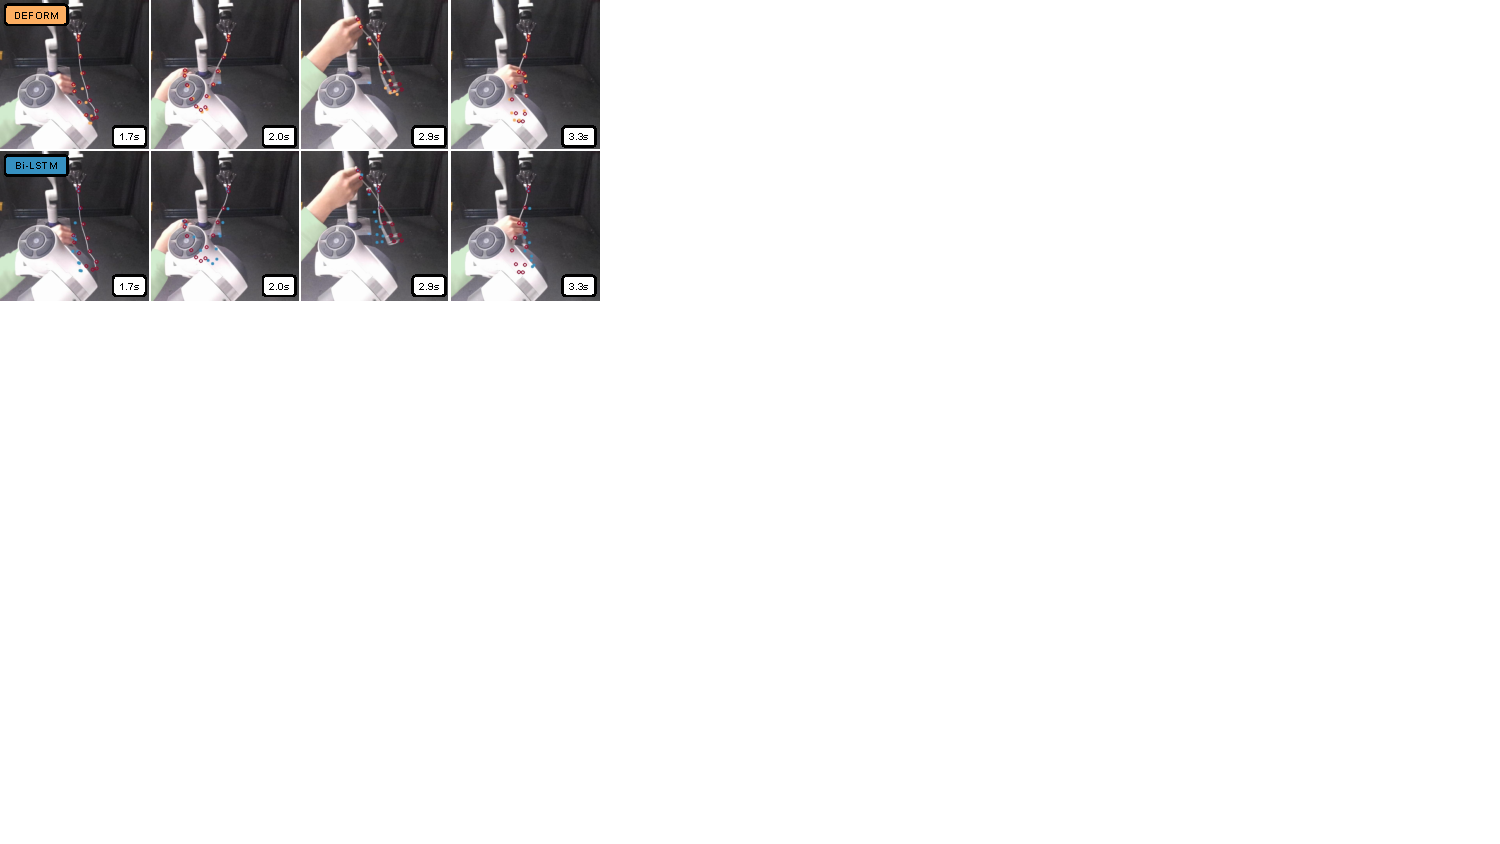
\includegraphics[width=\linewidth]{figures/exp_res_1.pdf}
%         \caption{DLO 1, robot-human manipulation}
%         \label{fig:rh_thin}
%     \end{subfigure}%
%     \hfill
%     \begin{subfigure}{0.49\textwidth}
%         \centering
%         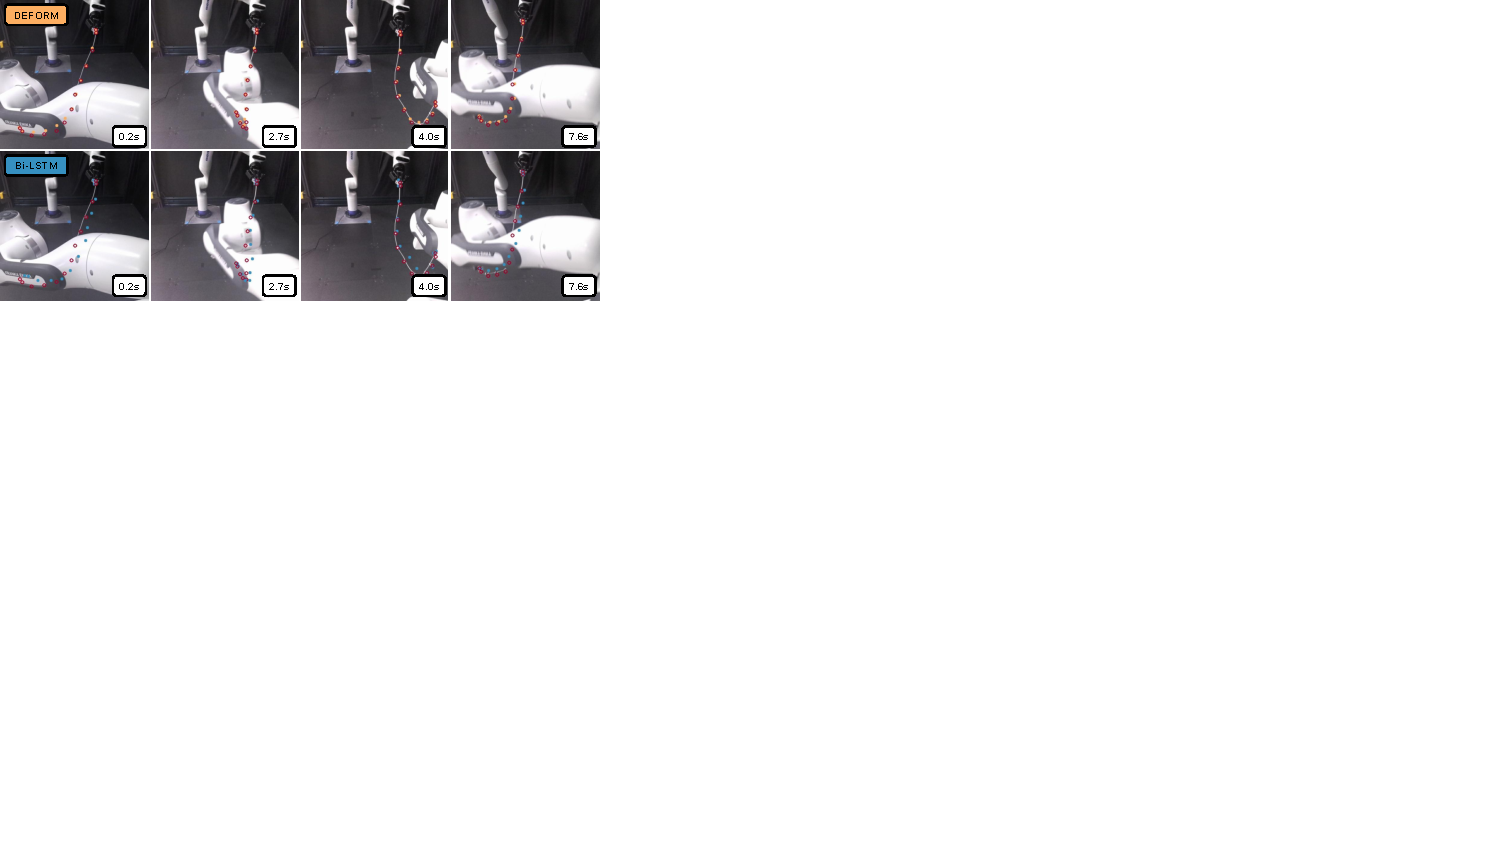
\includegraphics[width=\linewidth]{figures/exp_res_2.pdf}
%         \caption{DLO 1, dual-robot manipulation}
%         \label{fig:rr_thin}
%     \end{subfigure}
%     \vspace{0.2cm}

%     % Second row
%     \begin{subfigure}{0.49\textwidth}
%         \centering
%         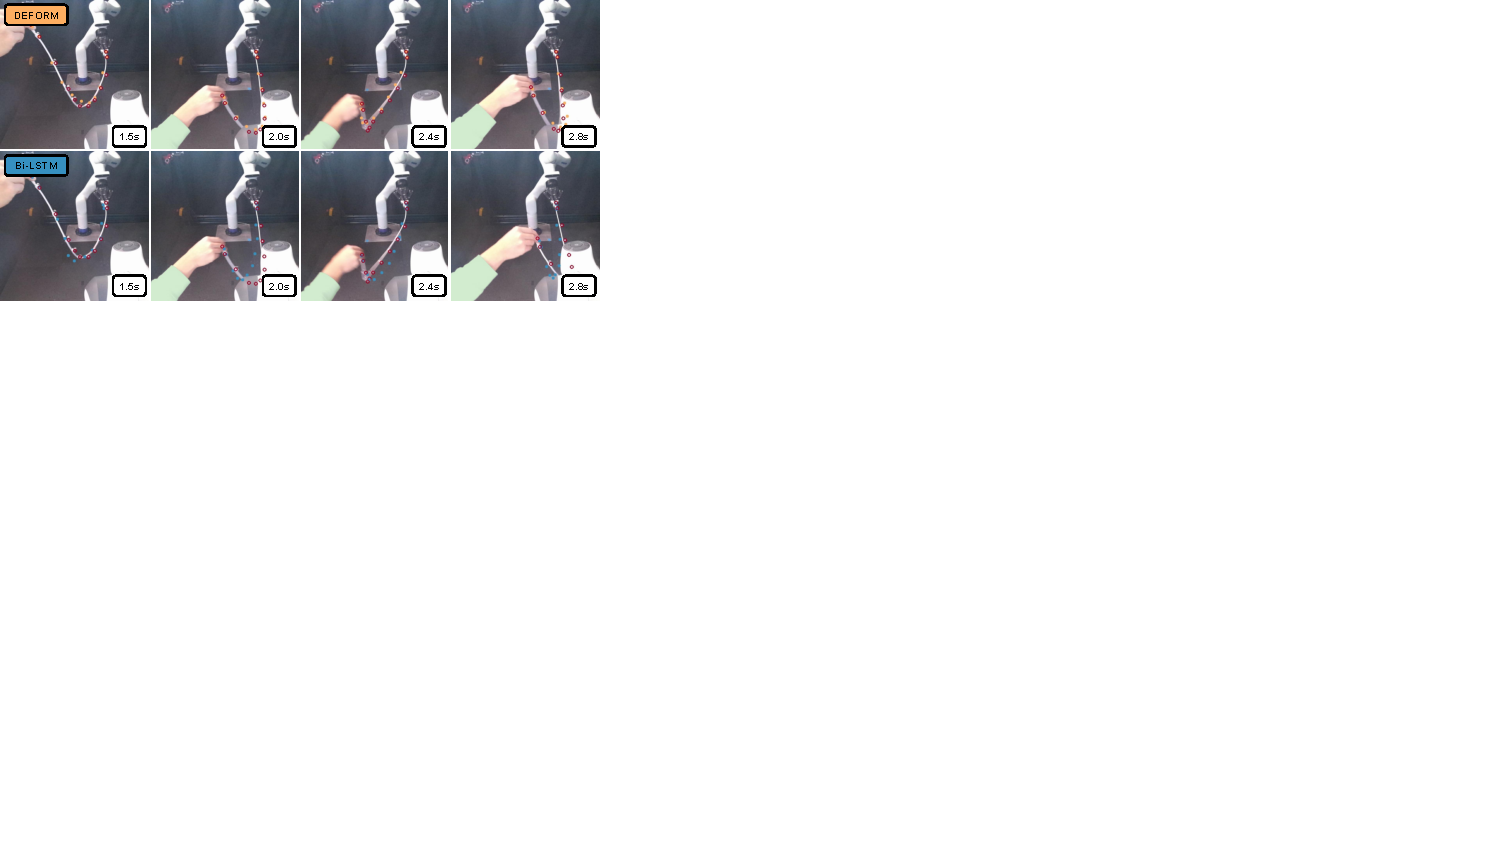
\includegraphics[width=\linewidth]{figures/exp_res_3.pdf}
%         \caption{DLO 2, robot-human manipulation}
%         \label{fig:rh_thick}
%     \end{subfigure}%
%     \hfill
%     \begin{subfigure}{0.49\textwidth}
%         \centering
%         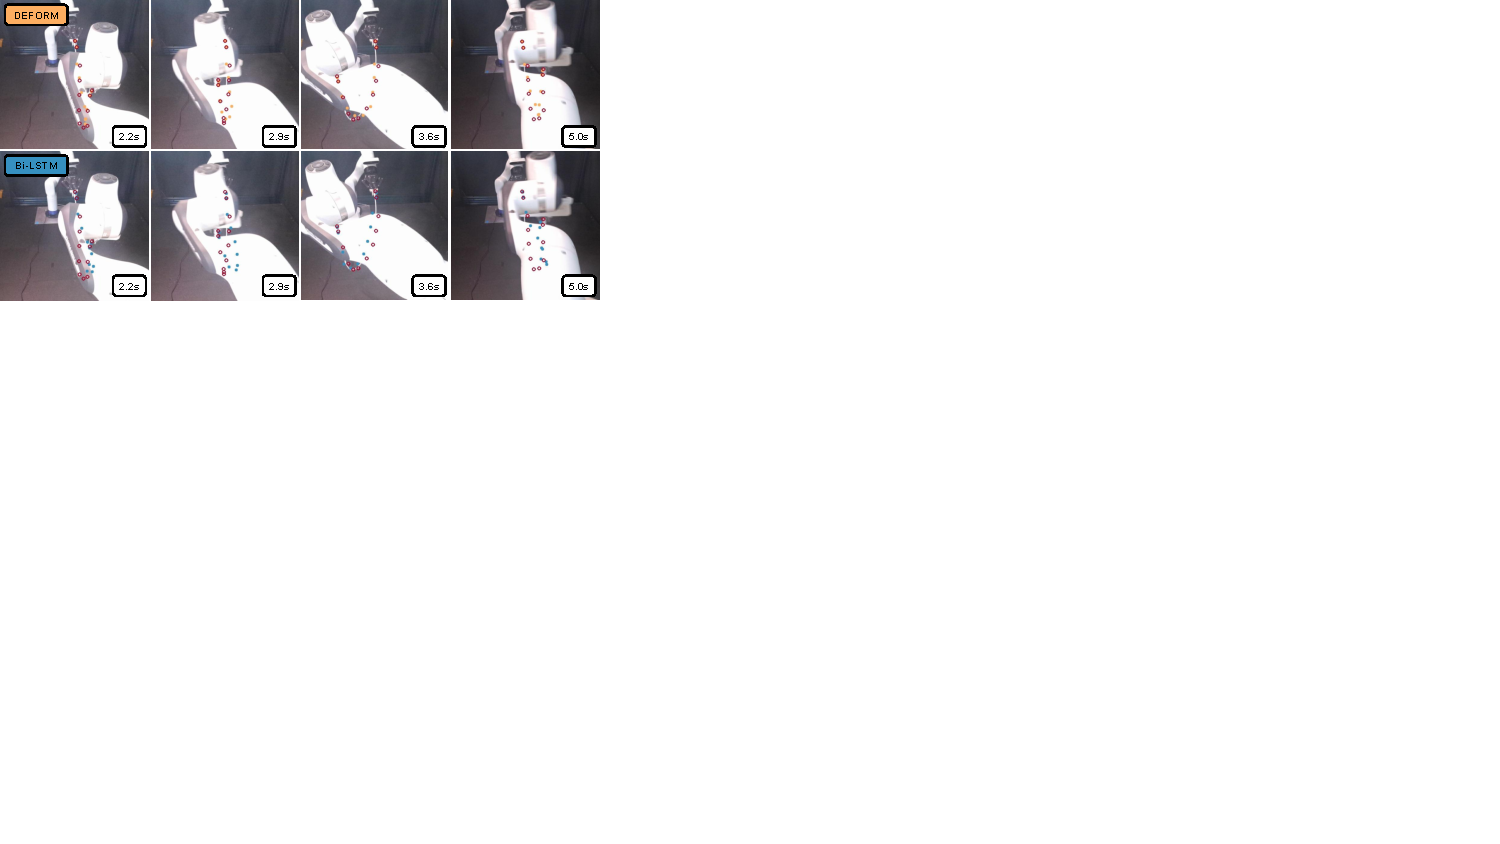
\includegraphics[width=\linewidth]{figures/exp_res_4.pdf}
%         \caption{DLO 2, dual-robot manipulation}
%         \label{fig:rr_thick}
%     \end{subfigure}
%     \vspace{0.2cm}

%     % Third row
%     \begin{subfigure}{0.49\textwidth}
%         \centering
%         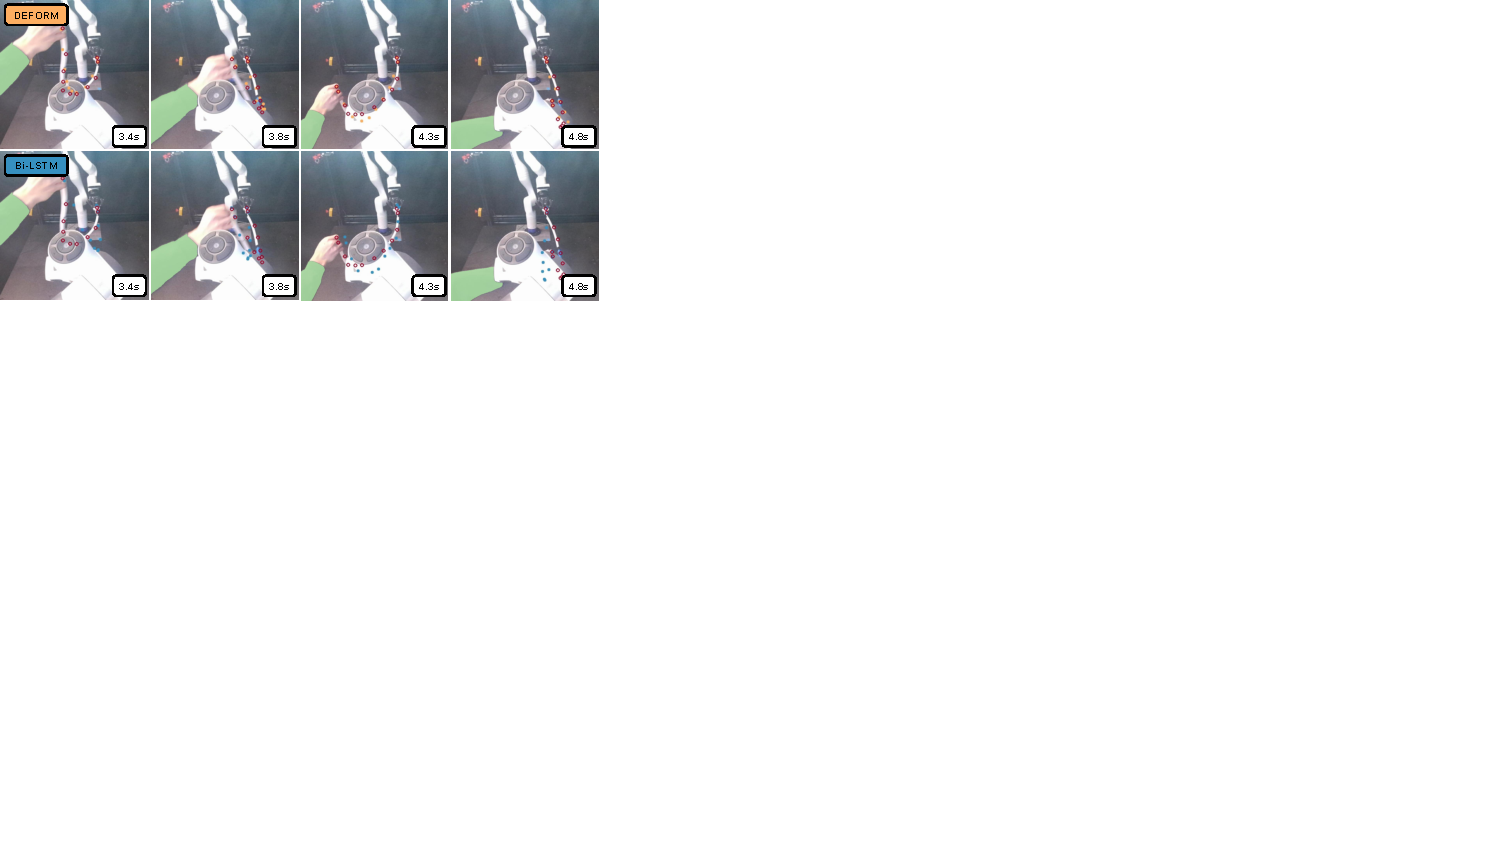
\includegraphics[width=\linewidth]{figures/exp_res_5.pdf}
%         \caption{DLO 3, robot-human manipulation}
%         \label{fig:rh_aniso}
%     \end{subfigure}%
%     \hfill
%     \begin{subfigure}{0.49\textwidth}
%         \centering
%         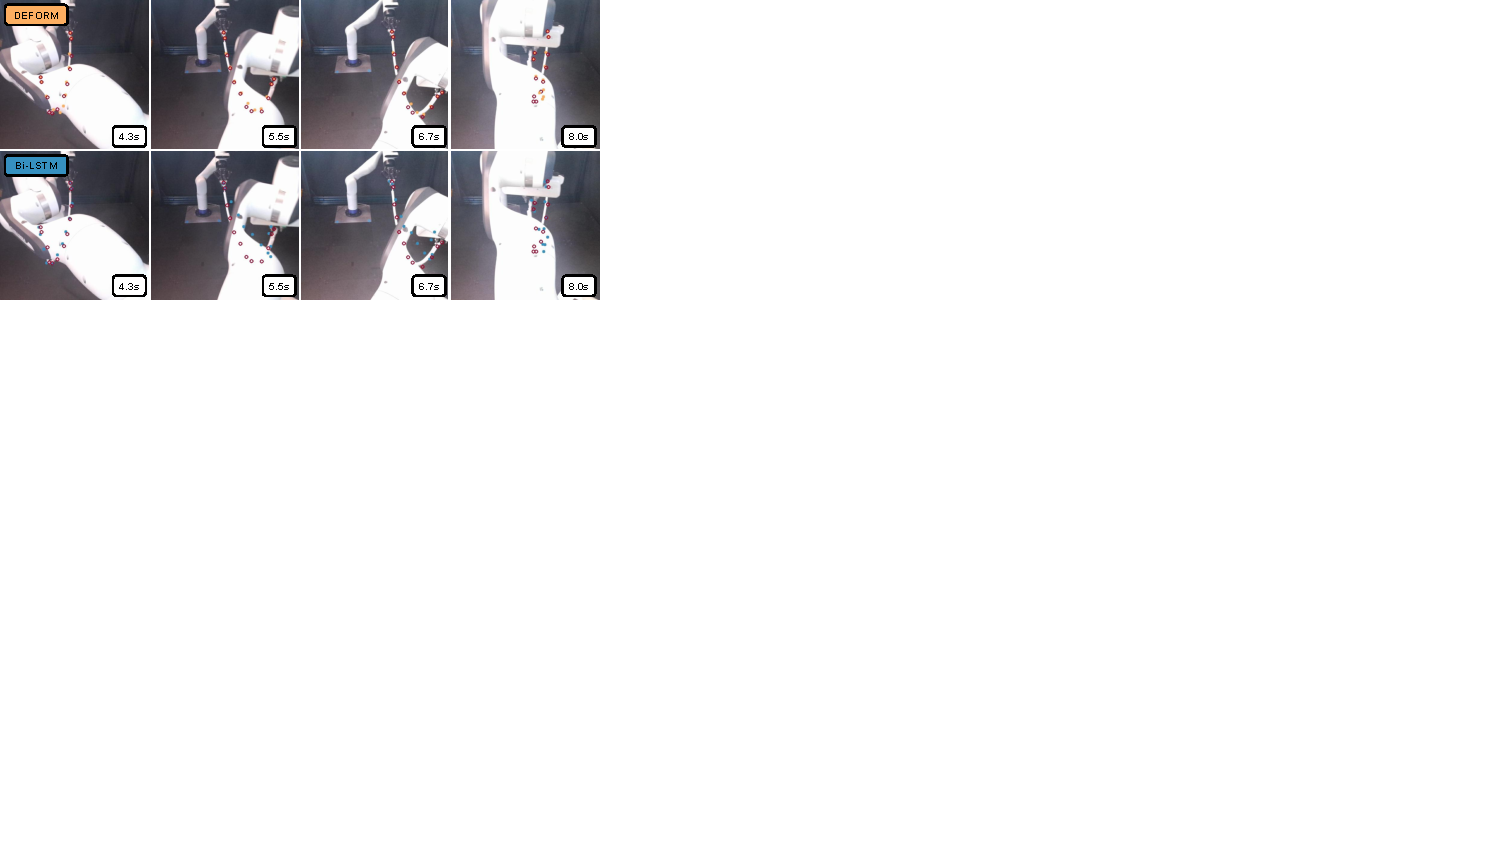
\includegraphics[width=\linewidth]{figures/exp_res_6.pdf}
%         \caption{DLO 3, dual-robot manipulation}
%         \label{fig:rr_aniso}
%     \end{subfigure}
%     \vspace{0.2cm}
%     \vspace{-0.2cm}

%     \caption{Visualization of the performance of DEFORM and Bi-LSTM in predicting trajectories for DLOs 1 \Revise{, 2, and 3}{}. The ground truth vertices of the DLOs are marked with red hollow circles. The predicted vertices are marked with orange solid circles for DEFORM and blue solid circles for the Bi-LSTM model, respectively.}
%     \label{fig:grid}
% \end{figure}